\chapter[SCP-130 邮局]{
    SCP-130 Post Office\\
    SCP-130 邮局
}

\label{chap:SCP-130}

\begin{figure}[H]
    \centering
    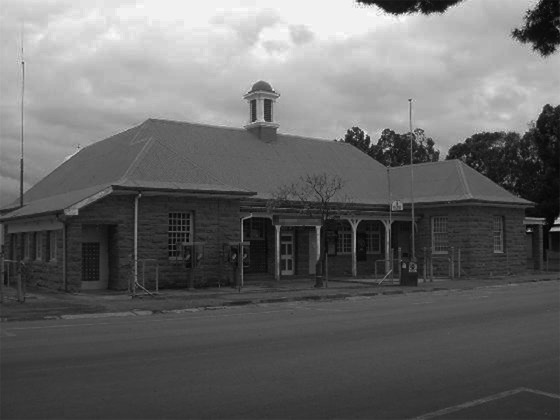
\includegraphics[width=0.5\linewidth]{images/SCP.130.jpg}
    \caption*{SCP-130}
\end{figure}

\bb{项目编号:}SCP-130

\bb{项目等级:}Euclid

\bb{特殊收容措施:}SCP-130必须每天进入工作时间两次,分别起始于当地日出前半小时和当地日落前半小时,每次由12名D级人员,6名2级安保特工和1名3级研究人员进行工作。他们必须身着特定制服\dd{并且必须是白人}。工作时间以外,必须有两名安保特工处于大厅,另有两名特工在建筑内巡视。若有人进入大厅,不建议特工进行阻拦,但若有人收取信件或包裹,应通知MTF Alpha-4("Pony Express")进行干预。

分拣室内每日会出现两次已打包的信件及包裹(SCP-130-2)。其中的包裹应由身着制服的工作人员分拣装袋并由特定的车辆运往Site-██。对寄往{[}删除]的信件,依Franklin-16(原文Franklin-Sixteen。以下还有Seventeen)流程处理,详见附录130-2;对其他信件进行标准检查。

若无O5-█许可,禁止在投寄口投入任何物品。Franklin-17流程描述了在此适用的处理方法。若其他任何人进入SCP-130使用投寄口,应当允许,随后MTF Alpha-4尽快干预并问讯。应检查此类事件之监控录像,追踪所投寄信件及其打包,并对比既有包裹列表。

\bb{描述:}SCP-130是一所邮局,位于南非████████,建于18██年,关闭于19██年,其后██年内处于废弃状态。尽管年久,该建筑保存极佳并免遭人类活动影响,甚至未有常规修缮。经与南非政府协议,SCP-130已被划为古迹。

每周有五日,在当地日出和日落时刻,邮局分拣室内会出现若干邮包和箱子。这些捆好的打包信件及包裹,即SCP-130-2,仅出现在周一至周五,当代的██邮政假日除外。其处理方法详见前述。

邮局大厅内除信箱外另有一标记为“寄出邮件”的投寄口,可投入最大宽40cm,高6cm的物品;就目前已知情况看来,没有长度限制。包裹一经投入便会消失,之后会出现在寄出邮件打包之中,除非之前已经历过这一步骤。

\bb{附录130-1:}SCP-130于19██年受到SCP基金会的注意。其时有盖着此地邮戳的国内与国际信件包裹在世界各地周转,均有足额邮资标记。

这些邮件通常无法寄达,原因或是收件地址不存在,或是收件人不在收件地址。它们被送至无着邮件中心。多名基金会人士注意到了邮戳奇异之处。于是MTF Alpha-4着手调查。他们抵达████████,发现城镇的大部分已荒废数十年,而邮局保养良好,并且清洁。

MTF Alpha-4搜查邮局之时,分拣室内出现了打包的邮件。特工们在检查中发现了各种各样的信函和包裹,并且全都注有当日日期以及该邮局邮戳。██████特工试图打开一个包裹,当即消失。六日后Site-██处的邮件分拣室出现一个邮包,内有██████特工,以及一信封,其上附有注明邮资不足的单据。处于昏迷的██████特工背上有“退回寄件人”和“邮资不足”字样文身。该信封被投入SCP-130投寄口时,██████特工方才苏醒,但对失踪期间毫无记忆。有其他特工试图带走、损坏包裹抑或破坏邮局,导致类似结果。

进一步的调查结果确立了现行收容措施,即要求\dd{白人}D级人员身着大约19██年时的█████ ████制服在邮件出现时进行分拣。邮件分拣完毕并被装入标有█████的车之后,即可平安载离此处。这些打包的邮件若无人处理,则会消失并在此后出现在世界各地的邮政部门之中以期投递。

\bb{附录130-2:}研究过去██年内的邮件,可以总结出一些特点。该邮局百分之██以上只是寻常邮件,不正常之处仅在于邮戳。其他邮件或是因各种原因未寄出,或是时空错乱。前者将会被销毁以维持SCP-130现状(尽管这么做有些奇怪);后者将接受检查,结果提交至{[}删除]。

寄往基金会成员或所属Site的信件应被统一送往Site-██以接受██████部门的检查。结果报告归于██████████项目之下,待O5人员审查。

Franklin-16流程:若收件人为{[}删除],则须将邮件密封于有主动反制设施的匣子内并送至当前5级监督处。在扫描排除爆炸、生化、模因或{[}删除]攻击的可能性后,将拆信并对其进行评估。目前收到的邮件尚未造成需要进行特殊收容的事态,但不可排除此种可能性。

寄往基金会的邮件所来自的时空是极其重要的因素,因此需要最小化其带来的影响。必须慎重评估利用邮件中的信息改变当前世界可能带来的负面影响。只有在O5人员投票达成2\slash 3多数时才可在当前时空利用SCP-130提供的信息影响当前世界进程。

\hyperref[sec:DOC-document-130-1]{档案130-1}中存放了拦截下的信息的样本。需要权限4\slash 130。

标有代码{[}删除]的邮件在扫描后必须不经5级人员而立即送往收件地址,并废除此代码,使用下一组。

Franklin-17流程:所有寄出邮件必须在寄出时付讫相当于████的邮资,并且标上代码{[}删除]。以这种方式寄出的邮件必须记录,并交叉对比以前的包裹以确保时空一致。

若试图寄件时出现标有邮资不足字样的单据,则应将补足的金额置于信封内并投入投寄口。可用的货币是兰特(南非货币单位)、欧元和██████████████(原文就是14个黑方块。前面的兰特和欧元都用了复数。有能力可以猜一下。反正我不知道)。使用伪钞会导致SCP-130采取致命的反应并要求罚金,直至邮件可以正常寄送。

\bb{附录130-3:}南非废除种族隔离后,SCP-130不再要求工作人员必须是白人。

\bb{事件130-6:}19██年██月█日,一件包裹送到了邮局。收件人为████ ███ ██████,收件地址为邮局内一信箱。当时被指派为SCP-130研究人员的█████博士将包裹投入了该邮箱,然后等待。██分钟后,████ ███ ██████略显困惑地走进大厅来到信箱旁。信箱在被他触摸的瞬间即解锁。他看到包裹上有自己的姓名时表现出了惊讶。

现场待命的MTF Alpha-4接到命令在该人离开SCP-130范围后立刻开始调查并对其进行讯问。该人当天本无计划来到████████,但在探访附近的家人时受到一股无从解释的强烈愿望的驱使,最终到来。当他打开包裹时,{[}删除]。该人受到A級记忆消除处理,之后接受记忆填充。

\newpage
\section{档案130-1}

\label{sec:DOC-document-130-1}

SCP-130-2样本执行总结。

至今日为止,共有█████件SCP-130-2样本依Franklin-16流程得到处理,除一定数量的例外,其他样本均被本部门检阅。以下是对于收件人为某几位基金会内外人士的邮件样本的总结。

M██████ █████ E██████博士,5\slash 130。

\hr

格式:

\bb{收件人:}█████\\
\bb{总结:}█████\\
\bb{备注:}█████

\hr

\bb{收件人:}Alto Clef博士\\
\bb{总结:}至今日为止,Clef博士一共收到了████件包裹,类型丰富,包括使用了Franklin-16中提到的代码的。这些包裹全都在以不同的方式尝试刺杀我们的好博士,并附有幸灾乐祸的、简洁的审判,甚至是道歉。\\
\bb{备注:}在造成了██人死亡以及令基金会蒙受价值███████美元的损失后,O5-█下令,要求所有收件人为Clef博士的邮件均必须接受严格的检查,并且必须依照“三号危险物质”规则遥控进行拆封。鉴于20██年█月██日的事件,对邮件的处理必须由D级人员进行,并在处理完毕前保持在50m范围内。

\bb{收件人:}Agatha Rights博士\\
\bb{总结:}寄给Rights博士的是各式贺卡,有生日贺卡,纪念日贺卡,还有其他的节日贺卡,比如寄自██████,██████ ██████和█████ █████的母亲节贺卡。\\
\bb{备注:}由于{[}删除],所有这些邮件均已焚毁,并且任何情况下都不应让Rights博士知晓。

\bb{收件人:}King博士\\
\bb{总结:}过去██年内,每年的植树节都会有与苹果有关的物品寄给King博士,包括苹果籽、苹果汁和白兰地。每年9月26日他还会收到John Chapman(又名Johnny Appleseed)的传记。\\
\bb{备注:}\ii{“天啊,这家伙对SCP-130做过什么?我觉得他根本就没去过南非!”}——5\slash 130

